
\chapter*{Chapter 5}
\markboth{Sprint 3 : Cartography \& Leaderboard }{Sprint 3 : Cartography \& Leaderboard} %pour afficher l'entete
 \addcontentsline{toc}{chapter}{5 Sprint 3 : Cartography \& Leaderboard}


\setcounter{chapter}{5}
\setcounter{section}{0}
\setcounter{table}{0} 
\setcounter{figure}{0} 


\etocsettocstyle{\subsection*{Plan}}{}
\vspace{0.25cm}

\setcounter{tocdepth}{1}
\headrule{
\vspace{0.5cm}

\begin{center}
    \textsc{\textbf {\Huge Sprint 3 : Cartography \& Leaderboard}} 
\end{center}
}
\headrule


\localtableofcontents
\newpage

\section*{Introduction}
Sprint 3 of our internship project involved creating the cartography and leaderboard modules for our network monitoring app.These features aim to provide an interactive map and an informative leaderboard to improve user engagement.Through this chapter we will discuss the analysis,the modeling and the realization of those modules.

\section{Sprint 3 Backlog}

The sprint backlog is a detailed list of tasks and user stories selected for completion within the current sprint, guiding the development team's work towards achieving the sprint goal. It serves as a dynamic, prioritized plan that evolves as the team progresses and new information emerges.
The table below describes the backlog of the third sprint :



\begin{table}[H]
    % \centering
    \renewcommand{\arraystretch}{1.2}
    \setlength{\belowcaptionskip}{0.25cm}
 
   \begin{tabular}{|p{0.05\textwidth}|p{0.2\textwidth}|p{0.34\textwidth}|p{0.34\textwidth}|}
   \hline
   \textbf{ID}  &  \textbf{User Story } & \textbf{Description} & \textbf{Task} \\ \hline


   
   \begin{center}
       \textbf{1}
   \end{center} & \begin{center}
       As a user, I want visualize different maps to have an idea about network condition
   \end{center} &
   \begin{center}
       
   The user can consult two types of map and visualize the different aspect of network conditions like average speed per county and networks availability across the country .
   \end{center}
   & 

       \begin{itemize}[left=0pt, label={\textbf{\Huge .}}]
       % \renewcommand\labelitemi{\textbf{\Huge .}}
            \item Create database to hold information about the entities involved (operator, kpi, cells, adm...)
            \item Develop module's backend 
            \item Develop the user interface for displaying data on the map 
        \end{itemize} \\ \hline


   \begin{center}
       \textbf{2}
   \end{center} & \begin{center}
       As a  user, I want to consult a leaderboard of best operator in my country
   \end{center} &
   \begin{center}
       
   
  The  user can visit a leaderboard of operators in his country and know the score of every operator in every time period  
   \end{center}
  & 

       \begin{itemize}[left=0pt, label={\textbf{\Huge .}}]
            \item Develop the user interface to display the leaderboard.
            \item Develop the database to hold information about operators score
            \item Develop the modules backend

        \end{itemize} \\ \hline
      
\end{tabular}
       \caption{Sprint 3 Backlog}
        \label{tab:my_label}
    
\end{table}



\newpage

\section{Sprint 2 use case diagram}

The figure below showcases the use case diagram for this sprint the involved actors and the expected functionalities  from our application.

\begin{figure}[H]
    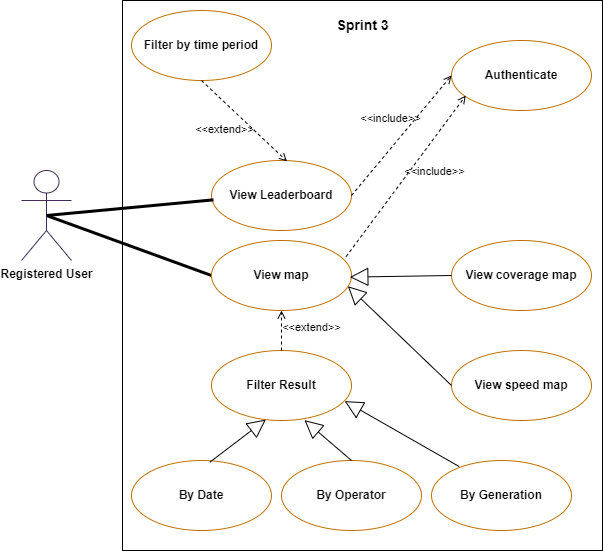
\includegraphics[width=0.98\textwidth]{images/sprint3/Sprint3UC.png}
     \caption{Sprint 3 Use Case Diagram}
    \label{fig:enter-label}
    
\end{figure}

\newpage
\section{User story n°1 : Cartography}
\textbf{\underline{Text description of the “View Map ” use case}}

\vspace{0.25cm}
We detail through this table the use case “View Map” :

\begin{table}[H]
    % \centering
    \renewcommand{\arraystretch}{1.5}
    
   \begin{tabular}{|p{0.25\textwidth}|p{0.72\textwidth}|}
   \hline
     
        \textbf{Use Case} & View map  \\   \hline
        
        \textbf{Actor(s) } &  Authenticated user   \\   \hline
        \textbf{Pre-condition} & 
              The User request the map page.
        \\  \hline
        \textbf{Post-condition} & None \\   \hline


                \textbf{Principal scenario} &
                \begin{enumerate}[left=0pt]
                    \item The user enter the desired parameter in the filter and submits.
                    \item The system load the corresponding map .
                    \item The system retrieves the requested data.
                    \item The system apply the data on the map .
                    \end{enumerate}  \\   \hline

                     \textbf{Alternative\newline scenario} & 
            If the requested data does not exist, an alert message appears to inform the user.
        \\   \hline
       
\end{tabular}

     \caption{Text Description Of The “View Map” Use Case}
    \label{tab:my_label}
    
\end{table}


\subsection{Sequence Diagram <<View map>> }



\begin{figure}[H]
   \begin{center}
    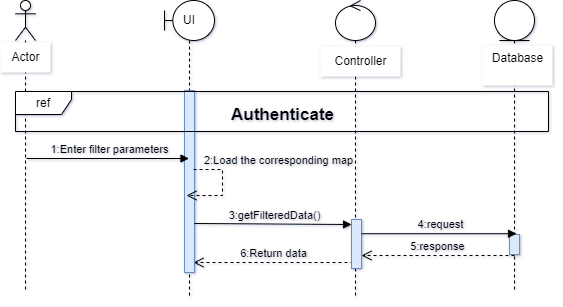
\includegraphics[width=\textwidth]{images/sprint3/cartographySeq.png}
    \caption{“View map” Sequence Diagram}
    \label{fig:enter-label}
   \end{center}
\end{figure}

\subsection{Sprint 2 Class Diagram}
\begin{figure}[H]
   
    
    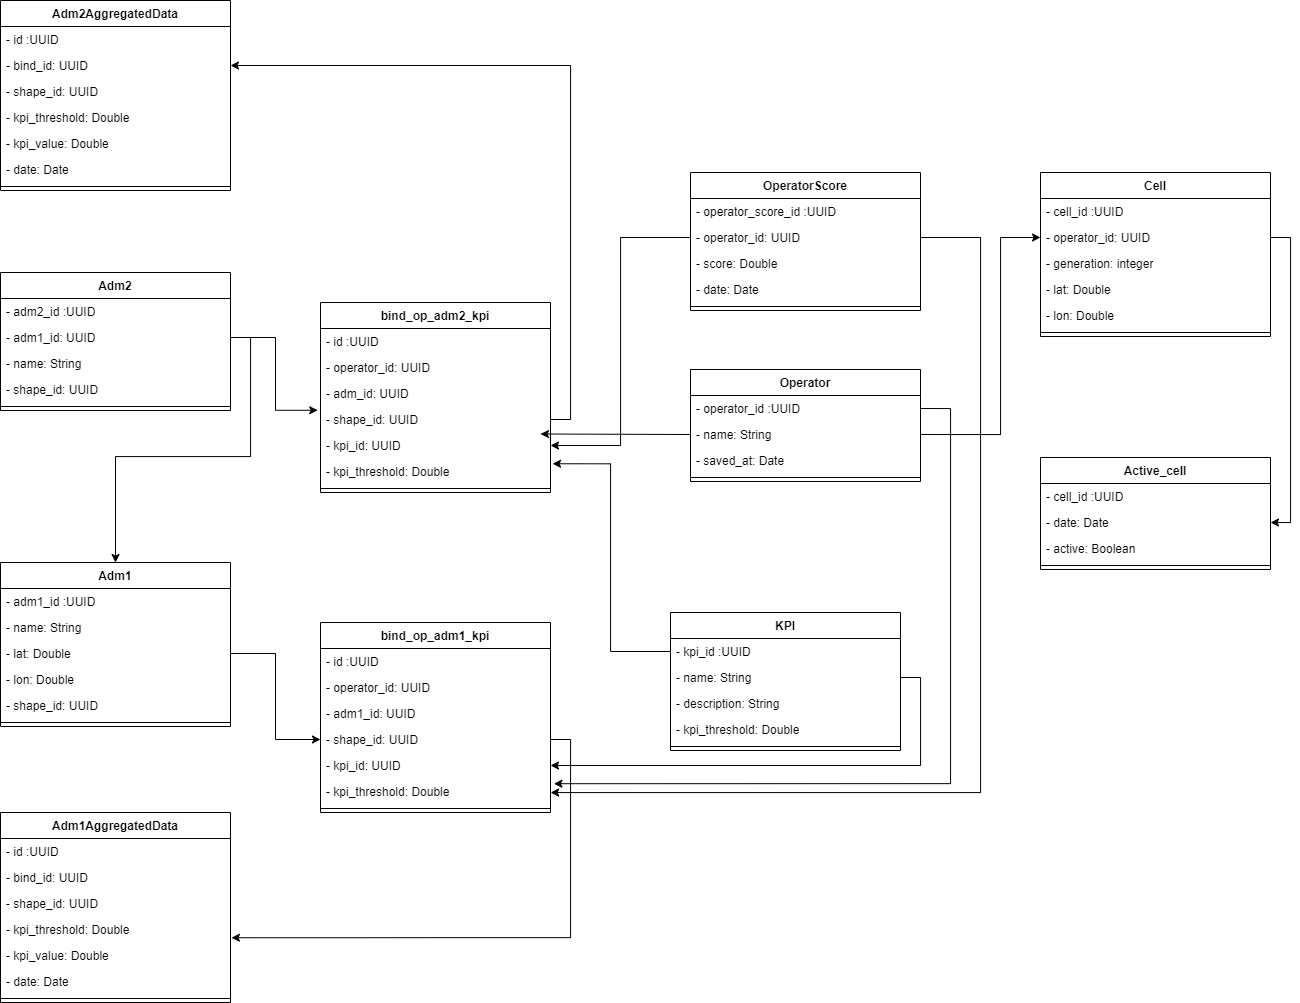
\includegraphics[width=\textwidth]{images/sprint3/Sprint3ClassDiag.png}
    \caption{Sprint 3 Class Diagram}
    \label{fig:enter-label}
    
\end{figure}
\newpage
\subsection{Realization}
In the section we will explore the final user interfaces related to the user story n°1 : "Cartography" in a sequential order :
\begin{figure}[H]
\begin{minipage}{0.32\textwidth}
    \centering
    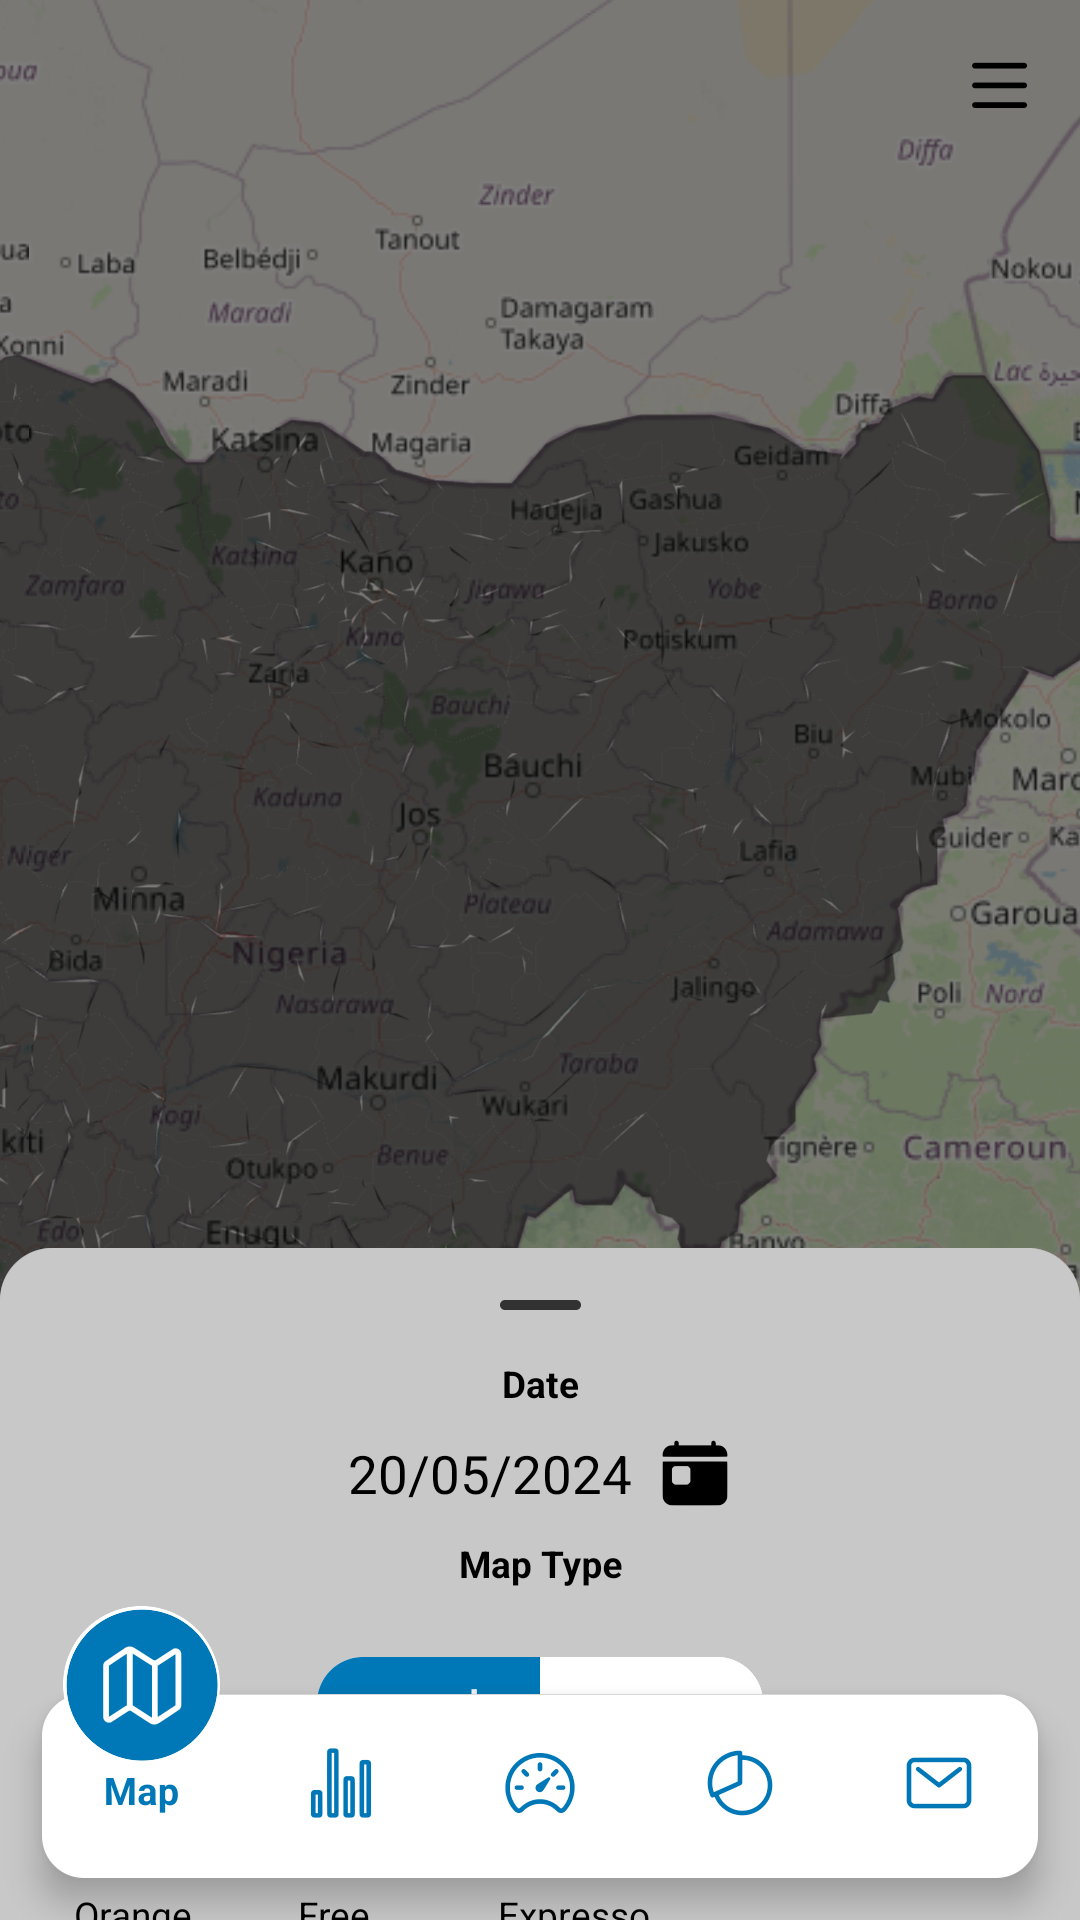
\includegraphics[width=\linewidth]{images/sprint3/mapModuleInit.png}
    \label{fig:login-form-filled}
\end{minipage}\hfill
\begin{minipage}{0.32\textwidth}
    \centering
    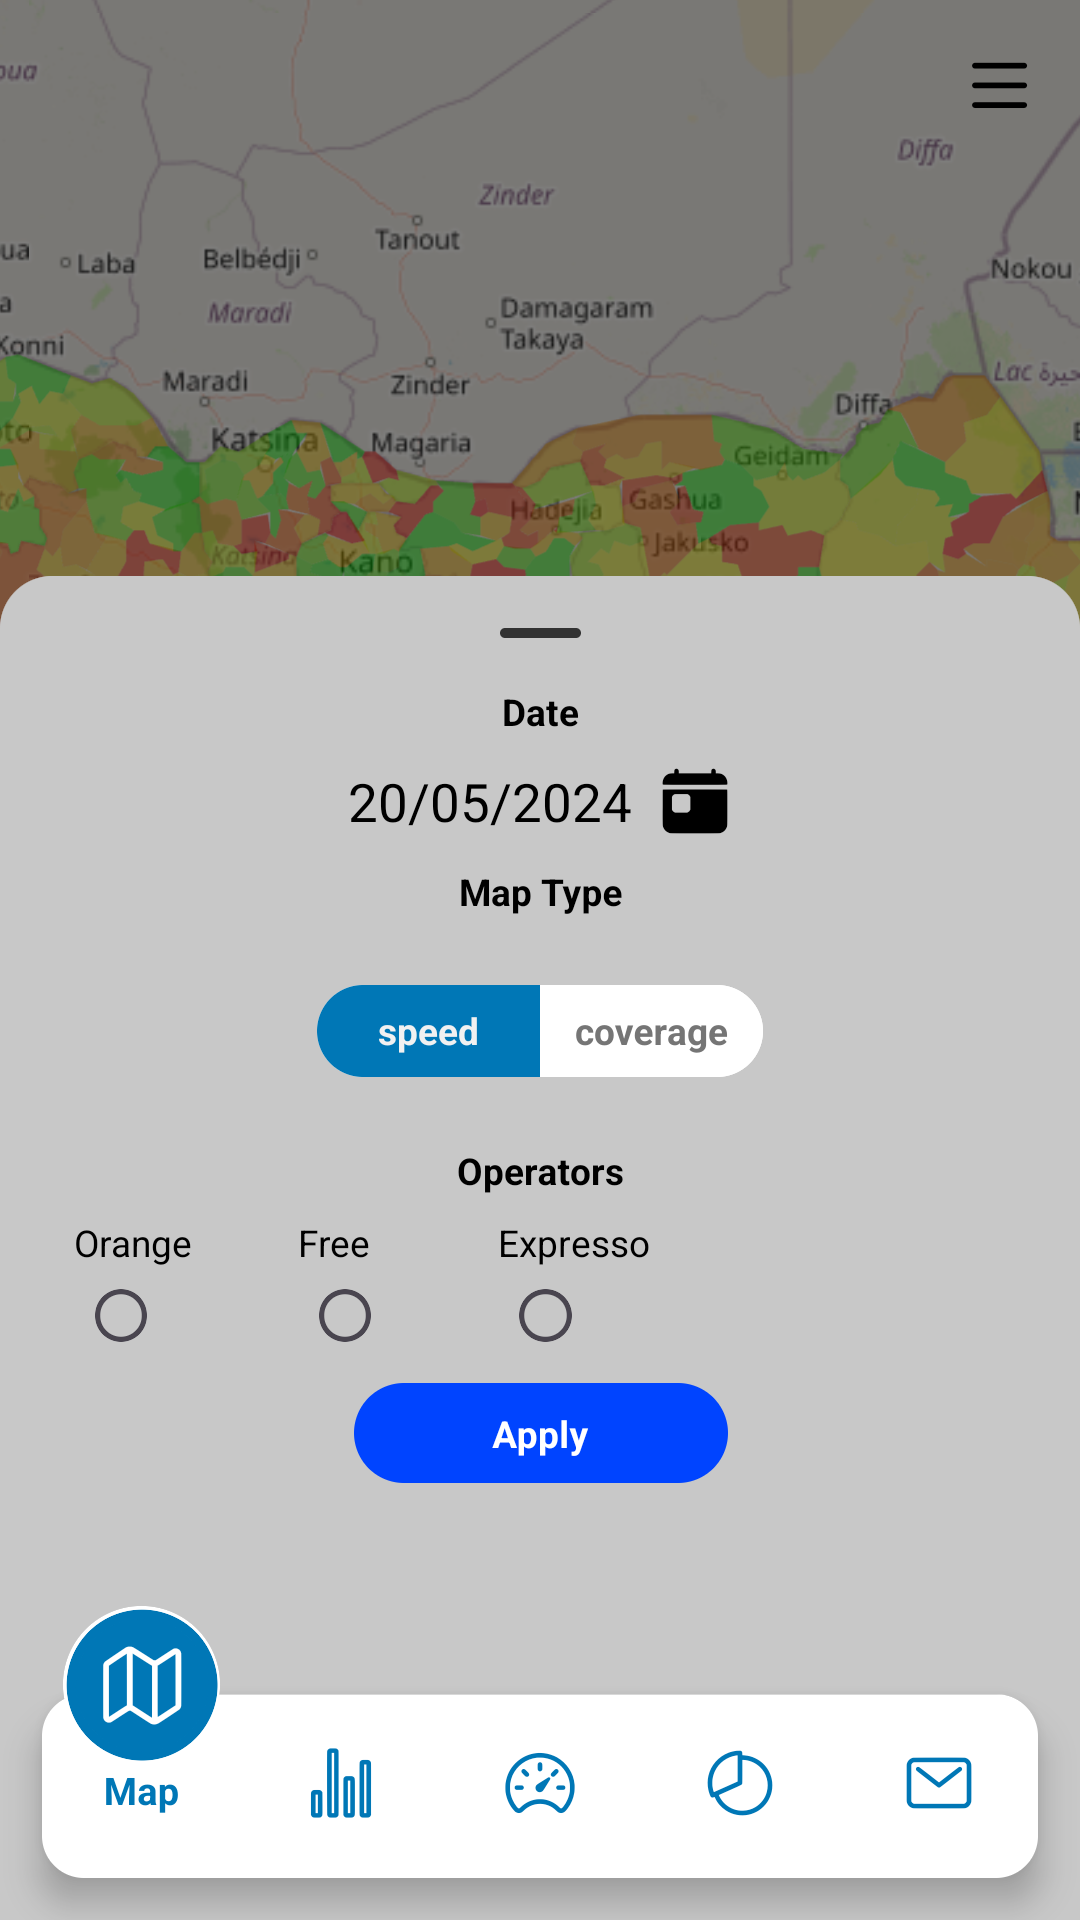
\includegraphics[width=\linewidth]{images/sprint3/speedFilter.png}
    \label{fig:login-form}
\end{minipage}\hfill
\end{figure}
% \newpage
% After Finishing the test a modal like shown in the screen shot below appears
\begin{figure}[H]
\begin{center}
    \begin{minipage}{0.32\textwidth}
    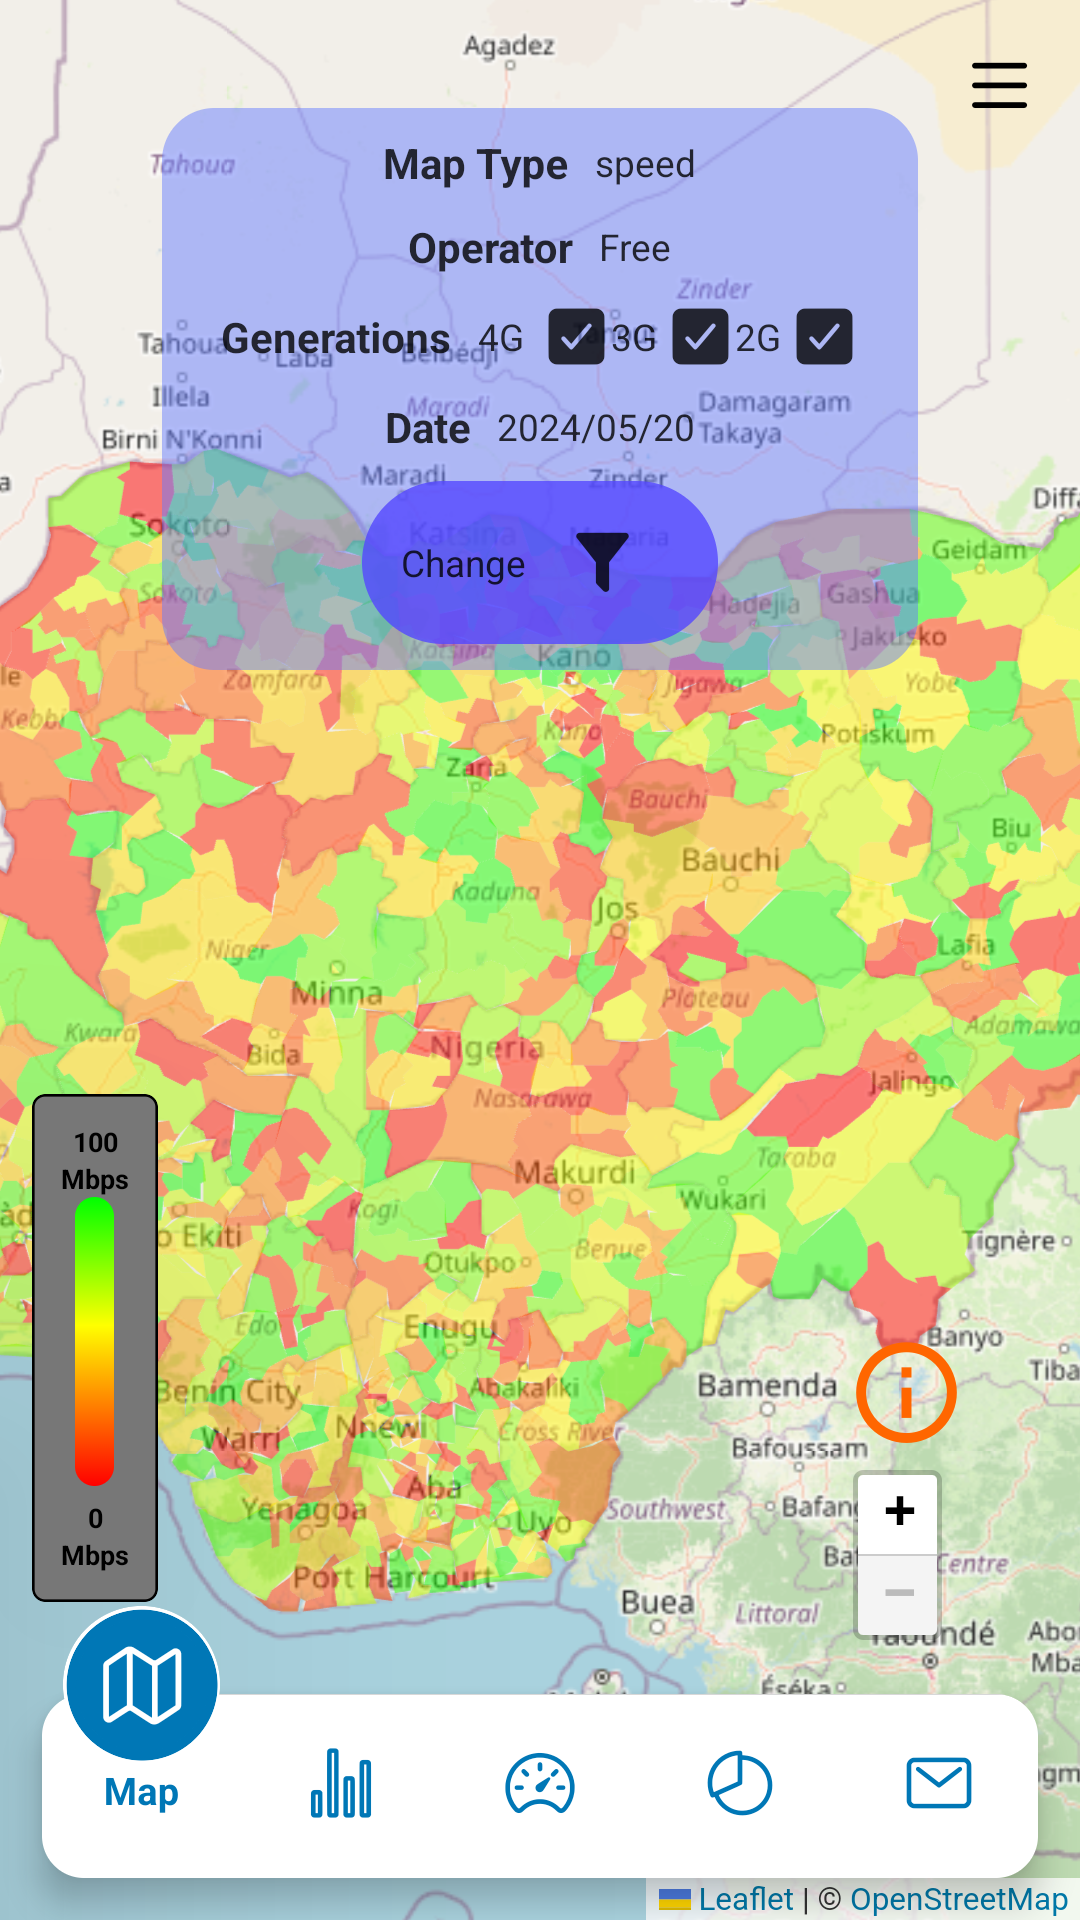
\includegraphics[width=\textwidth]{images/sprint3/speedMapWithInfo.png}
    \label{fig:enter-label}
    \end{minipage}\hfill
    \caption{Speed Map}
\end{center}
\end{figure}


\newpage
\section{User story n°2 : Leaderboard}

\textbf{\underline{Text description of the “View Leaderboard”use case:}}

\vspace{0.25cm}

We detail through this table the use case “View Leaderboard” :

\begin{table}[H]
    % \centering
    \renewcommand{\arraystretch}{1.5}
    
   \begin{tabular}{|p{0.25\textwidth}|p{0.68\textwidth}|}
   \hline
     
        \textbf{Use Case} & View Leaderboard  \\   \hline
        
        \textbf{Actor(s) } & Authenticated User  \\   \hline
        \textbf{Pre-condition} & The user requests the leaderboard screen \\   \hline
        \textbf{Post-condition} & None  \\   \hline
                \textbf{Principal scenario} & 
                \begin{enumerate}
                    \item The system serves the leaderboard screen with default filter applied
                    \item The user change the time period.
                    \item The system retrieves the data.
                    \item The user interface updates the values.
                \end{enumerate}  \\   \hline
        
        \textbf{Alternative\newline scenario} & 
        \begin{center}
        None
        \end{center}
         \\   \hline
\end{tabular}
     \caption{Text Description Of The “View Leaderboard” Use Case}
    \label{tab:my_label}
\end{table}


\newpage

\subsection{Sequence Diagram<<View Leaderboard>> }
Below, we present the sequence diagrams for each use case mentioned above.

\begin{figure}[H]
   
    
    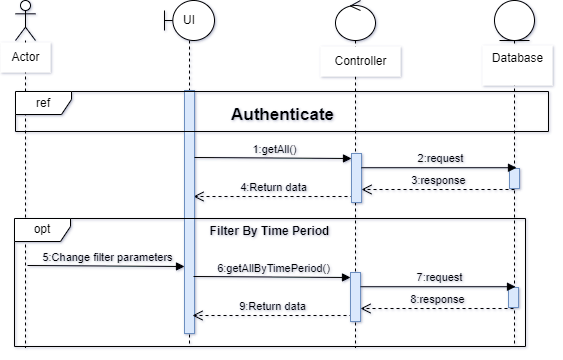
\includegraphics[width=0.98\textwidth]{images/sprint3/leaderboardSeq.png}
    \caption{"View Leaderboard" sequence diagram}
    \label{fig:enter-label}
    
\end{figure}
% Realization
\subsection{Realization}
In this section we will showcase the final outcome of the second user story of this sprint :
\begin{figure}[H]
\begin{minipage}{0.3\textwidth}
    \centering
    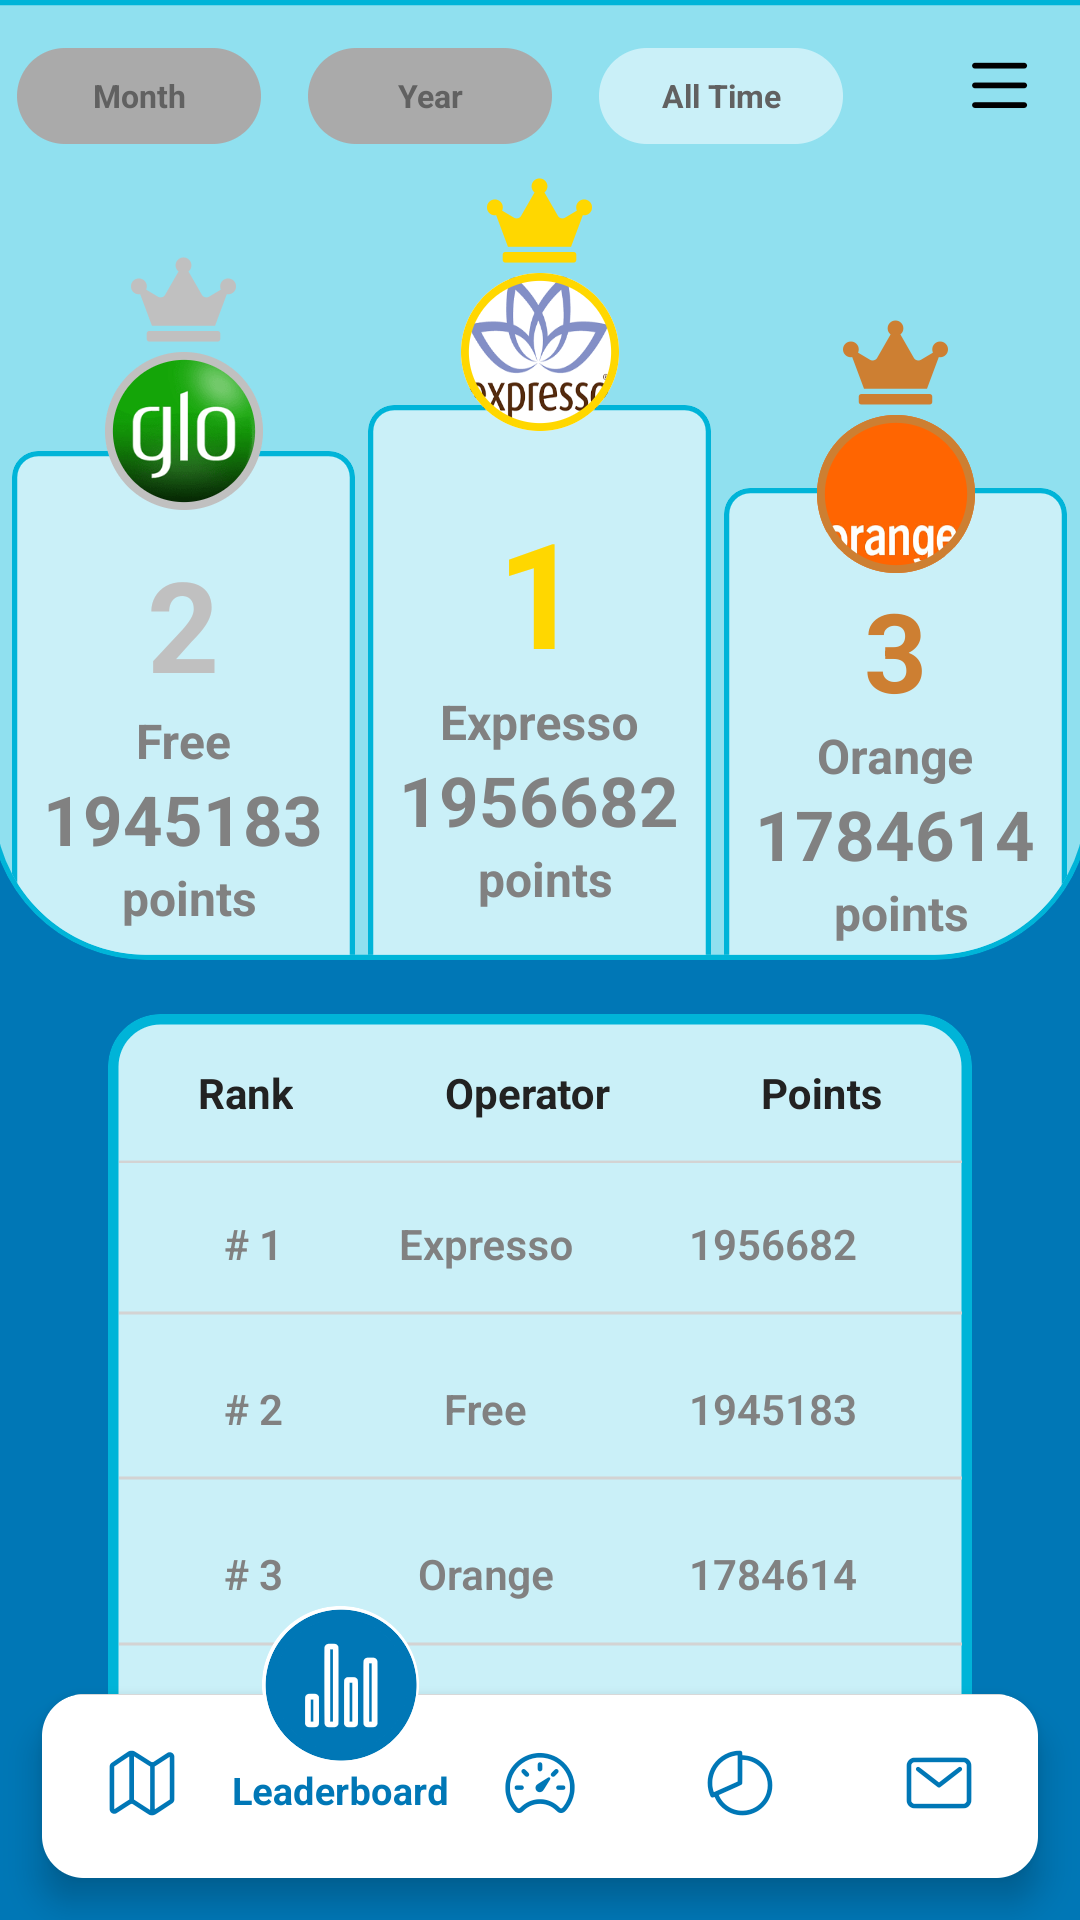
\includegraphics[width=\linewidth]{images/sprint3/leaderBoardModule (3).png}
    \label{fig:login-form-filled}
\end{minipage}\hfill
\begin{minipage}{0.3\textwidth}
    \centering
    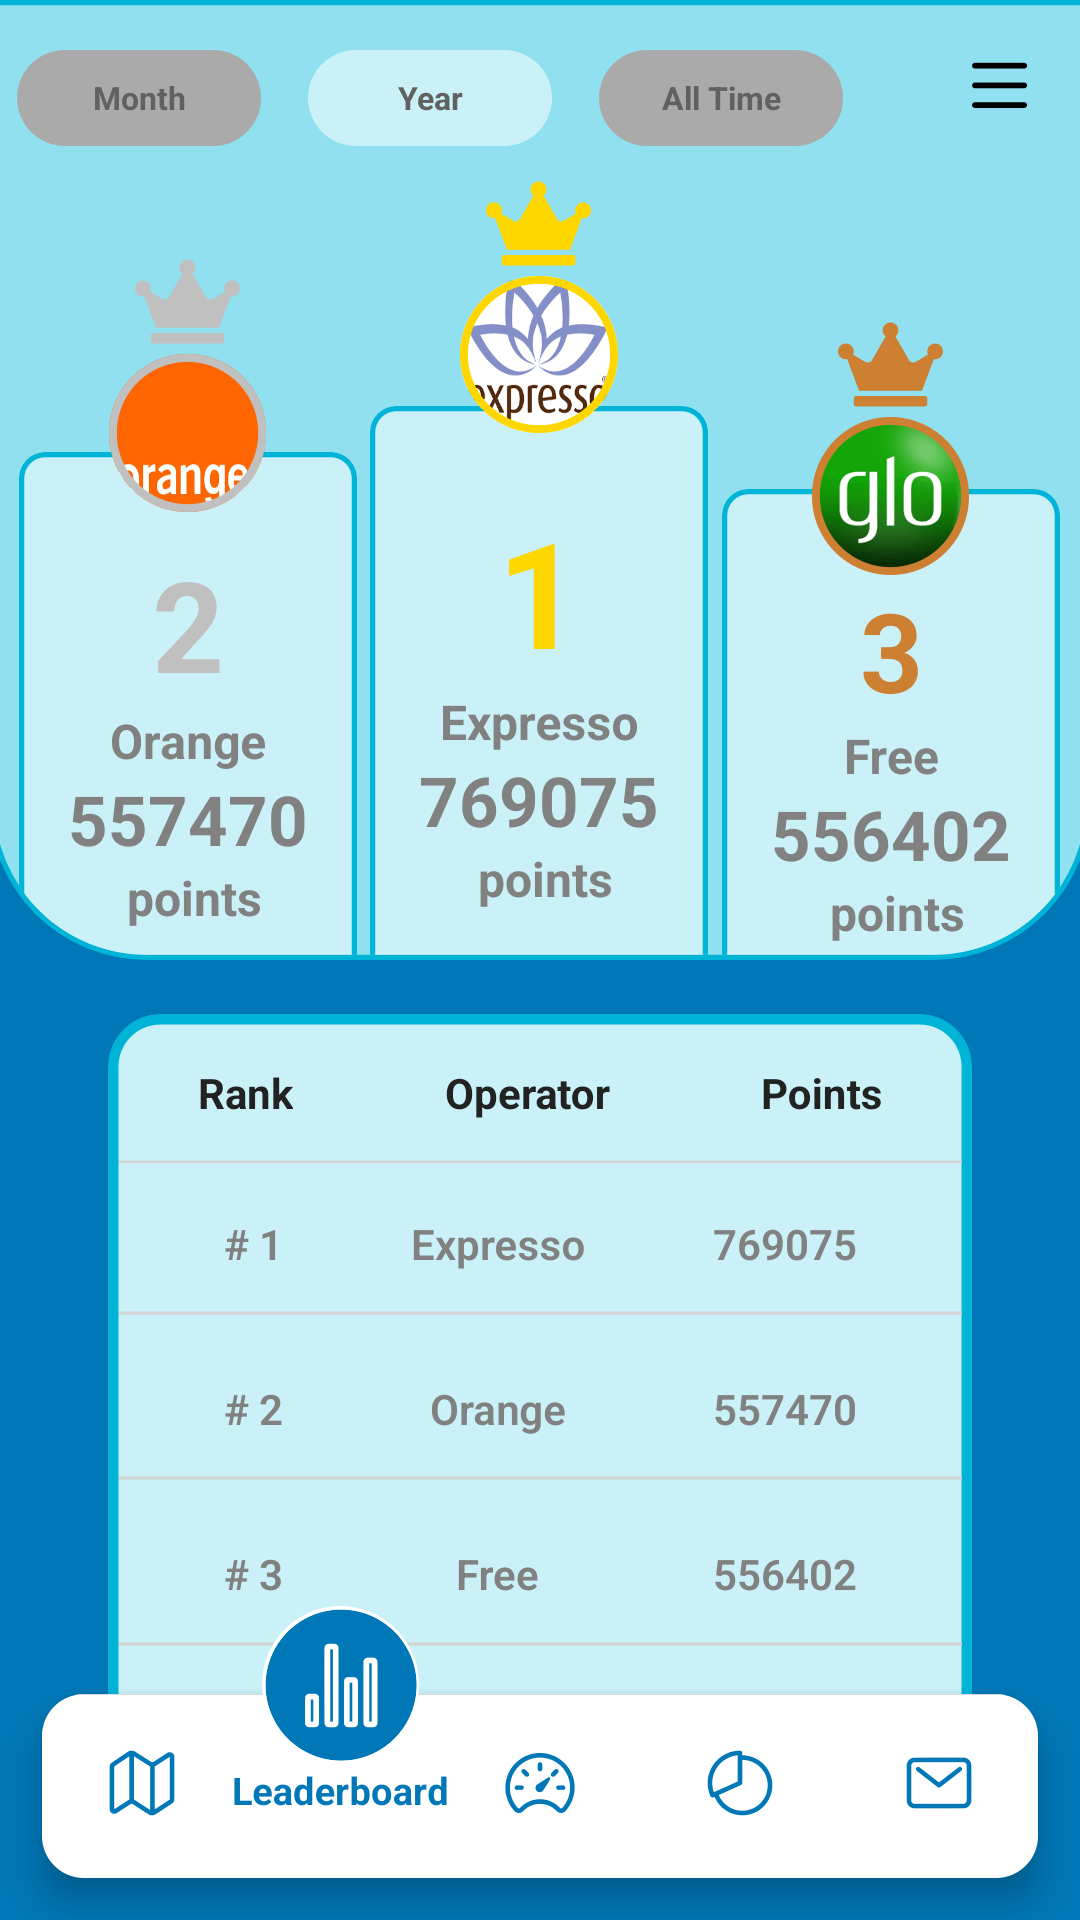
\includegraphics[width=\linewidth]{images/sprint3/leaderBoardModule (2).png}
    % \caption{Forget Password Sequence Diagram Part 1}
    \label{fig:login-form}
\end{minipage}\hfill
    % \caption{Reports Screen}
\end{figure}
\begin{center}
    
\begin{figure}[H]
    \centering
    % \caption{Forget Password Sequence Diagram Part 1}
    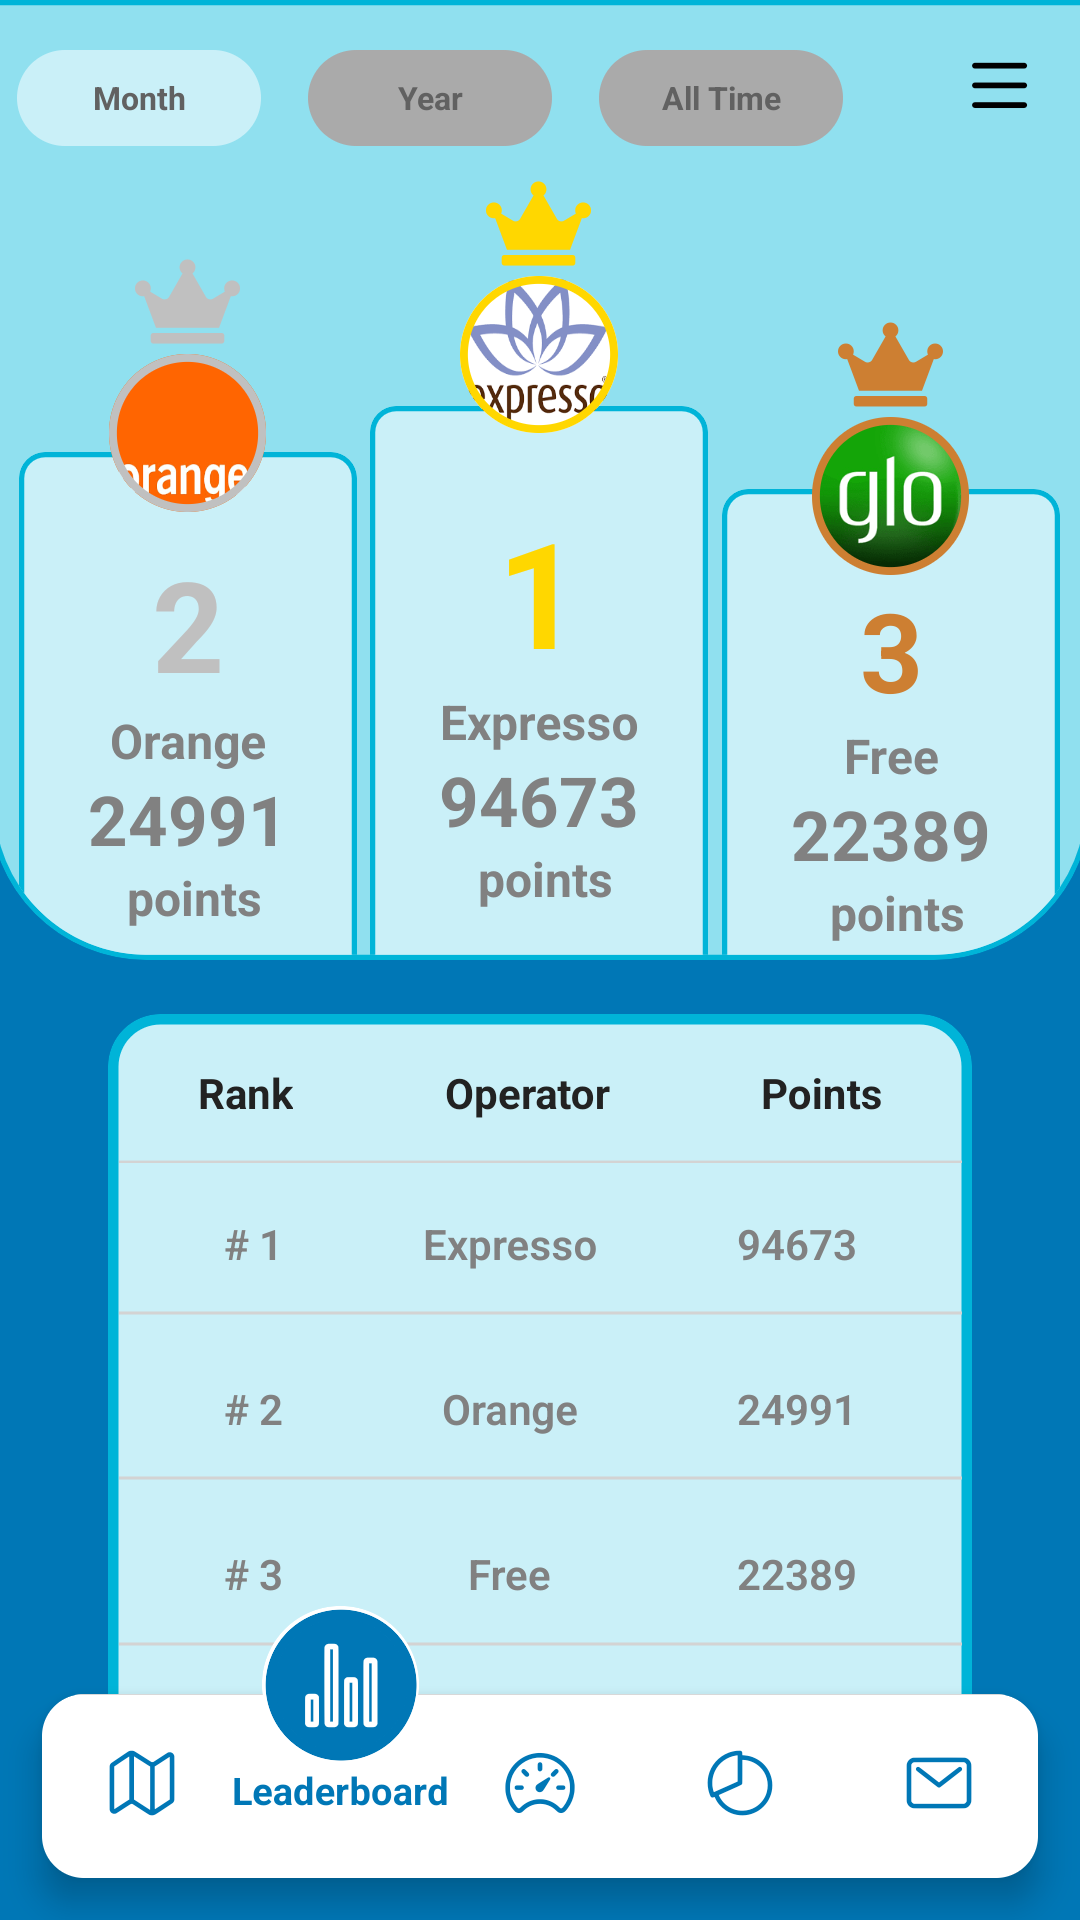
\includegraphics[width=0.3\linewidth]{images/sprint3/leaderBoardModule (1).png}
    \label{fig:login-form}
    \caption{Leaderboard screen}
\end{figure}
\end{center}


\section*{Conclusion}

By the end of this sprint, we successfully overcame the challenges encountered and added a significant enhancement to our application. In the next chapter, we will delve into the "Reviews \& Feedback" module, continuing to build on our progress.
